Trong phần này, chúng tôi trình bày các thực nghiệm để chứng minh tính hiệu quả của MAGNN đối với việc biểu diễn đồ thị không đồng nhất. Các thực nghiệm nhằm giải quyết các câu hỏi nghiên cứu sau:

\begin{itemize}
  \item RQ1. MAGNN có hiệu quả như thế nào trong việc phân loại các nút?
  \item RQ2. MAGNN có hiệu quả như thế nào trong việc phân cụm các nút?
  \item RQ3. MAGNN có hiệu quả như thế nào trong việc dữ đoán các liên kết hợp lí giữa các cặp nút?
  \item RQ4. Ảnh hưởng của 3 thành phần chính của MAGNN đã được mô tả trong các phần trước đó là gì?
  \item RQ5. Làm cách nào để ta có thể xác định được tính đại diện của những phương pháp biểu diễn đồ thị khác nhau?
\end{itemize}

\subsection{Tập dữ liệu}
Chúng tôi lựa chọn 03 tập dữ liệu đồ thị không đồng nhất phổ biến nhất hiện nay từ các lĩnh vực khác nhau để đánh giá hiệu năng của MAGNN khi so sánh với các phương pháp cơ sở là các phương pháp tối ưu nhất hiện nay (baselines). Cụ thể, tập dữ liệu IMDb và DBLP được sử dụng trong thực nghiệm liên quan đến việc phân loại nút và phân cụm nút. Tập dữ liệu Last.fm được sử dụng cho thực nghiệm về khả năng dự báo mối quan hệ. Những giá trị thống kê cơ bản của 03 tập dữ liệu được tóm tắt trong Bảng 2, và mô hình mạng được thể hiện trong Hình 3. Chúng tôi sử dụng vector one-hot cho các nút không có thuộc tính như là các thuộc tính đầu vào giả (dummy) của chúng. 

\begin{figure*}
  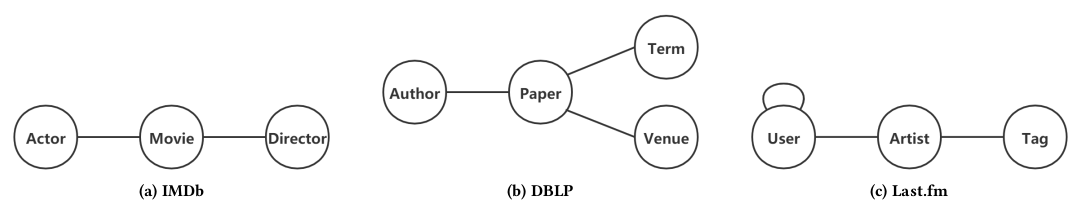
\includegraphics[width=\textwidth]{figs/fig3.png}
  \caption{Các lược đồ mạng của ba bộ dữ liệu đồ thị không đồng nhất được sử dụng trong bài viết này.}
\end{figure*}

\begin{itemize}
  \item $\mathbf{IMDb}^{1}$ là cơ sở dữ liệu trực tuyến về các bộ phim và chương trình truyền hình, bao gồm các thông tin như dàn diễn viên, đội ngũ sản xuất và tóm tắt cốt truyện. Chúng tôi sử dụng một tập mẫu được lấy ra từ IMDb, thông qua quá trình tiền xử lí dữ liệu thu được 4278 bộ phim, 2081 đạo diễn và 5257 diễn viên. Phim được gắn nhãn là một trong ba loại (Hành động, Hài kịch và Chính kịch) dựa trên thông tin thể loại của chúng. Mỗi bộ phim cũng được mô tả bằng một bag-of-words đại diện cho các từ khóa cốt truyện của chúng. Đối với các mô hình học bán giám sát, các nút phim được chia thành các tập huấn luyện, xác thực và kiểm tra với kích thước lần lượt là 400 (9,35\%), 400 (9,35\%) và $3478(81,30 \%)$ nút.
  \item $\mathbf{DBLPP}^{2}$ là một trang web tổng hợp danh mục tài liệu về khoa học máy tính. Chúng tôi sử dụng một tập mẫu được lấy ra từ DBLP [12, 15], sau khi tiền xử lí dữ liệu thu được thông tin về 4057 tác giả, 14328 bài báo, 7723 thuật ngữ và 20 nơi xuất bản. Các tác giả được chia thành bốn lĩnh vực nghiên cứu (Cơ sở dữ liệu, Khai thác dữ liệu, Trí tuệ nhân tạo và Truy xuất thông tin). Mỗi tác giả được mô tả bằng một bag-of-words đại diện cho các từ khóa trong bài báo của họ. Đối với các mô hình học bán giám sát, các nút tác giả được chia thành các tập huấn luyện, xác thực và kiểm tra với kích thước lần lượt là $400(9,86 \%)$ 400 (9,86\%) và 3257 (80,28\%) nút.
  \item $\mathbf{Last.fm}^{3}$ là trang web âm nhạc theo dõi thông tin hành vi nghe nhạc của người dùng từ nhiều nguồn khác nhau. Chúng tôi sử dụng bộ dữ liệu do HetRec 2011 phát hành [4], sau khi tiền xử lí dữ liệu thu được thông tin về 1892 người dùng, 17632 nghệ sĩ và 1088 thẻ nghệ sĩ. Tập dữ liệu này được sử dụng cho tác vụ dự đoán liên kết giữa các nút, trong đó tập dữ liệu không chưa bất cứ thông tin nào liên quan đến nhãn hay các đặc điểm đặc trưng của đối tượng. Đối với các mô hình học bán giám sát, các cặp người dùng-nghệ sĩ được chia thành các tập huấn luyện, xác thực và kiểm tra với kích thước lần lượt là $64984(70 \%), 9283(10 \%)$ và $18567(20 \%)$ cặp.
\end{itemize}

\subsection{Các mô hình tham chiếu}
Chúng tôi so sánh MAGNN với nhiều loại mô hình biểu diễn đồ thị khác nhau, bao gồm các mô hình biểu diễn đồ thị đồng nhất truyền thống (trái ngược với GNN), mô hình biểu diễn đồ thị không đồng nhất truyền thống, GNN cho đồ thị đồng nhất và GNN cho đồ thị không đồng nhất. Ta gọi chúng lần lượt là mô hình đồng nhất truyền thống, mô hình không đồng nhất truyền thống, GNN đồng nhất và GNN không đồng nhất. Danh sách các mô hình cơ sở được thể hiện dưới đây.

\begin{table}[]
  \label{tb:02}
  \caption{Thống kê mô tả các tập dữ liệu}
  \begin{tabular}{|l|l|l|l|}
  \hline
  Dữ liệu & Nút                                                                                                                                     & Cạnh                                                                                     & Metapath                                                                      \\ \hline
  IMDb    & \begin{tabular}[c]{@{}l@{}}\# phim (M): 4278\\ \# đạo diễn (D): 2081\\ \# diễn viên (A): 5257\end{tabular}                              & \begin{tabular}[c]{@{}l@{}}\# M-D: 4278\\ \# M-A: 12828\end{tabular}                     & \begin{tabular}[c]{@{}l@{}}MDM\\ MAM\\ DMD\\ DMAMD\\ AMA\\ AMDMA\end{tabular} \\ \hline
  DBLP    & \begin{tabular}[c]{@{}l@{}}\# tác giả (A): 4057\\ \# bài báo (P): 14328\\ \# thuật ngữ (T): 7723\\ \# nới xuất bản (V): 20\end{tabular} & \begin{tabular}[c]{@{}l@{}}\# A-P: 19645\\ \# P-T: 85810\\ \# P-V: 14328\end{tabular}    & \begin{tabular}[c]{@{}l@{}}APA\\ APTPA\\ APVPA\end{tabular}                   \\ \hline
  Last.fm & \begin{tabular}[c]{@{}l@{}}\# người dùng (U): 1892\\ \# nghệ sĩ (A): 17632\\ \# thẻ (T): 1088\end{tabular}                              & \begin{tabular}[c]{@{}l@{}}\# U-U: 12,717\\ \# U-A: 92,834\\ \# A-T: 23,253\end{tabular} & \begin{tabular}[c]{@{}l@{}}UU\\ UAU\\ UATAU\\ AUA\\ AUUA\\ ATA\end{tabular}   \\ \hline
  \end{tabular}
  \end{table}

\begin{itemize}
  \item $\mathbf{LINE}$ [25] là một mô hình đồng nhất truyền thống khai thác mức độ tương đồng bậc nhất và bậc hai giữa các nút. Chúng tôi áp dụng mô hình này cho các đồ thị không đồng nhất bằng cách bỏ qua tính không đồng nhất của cấu trúc đồ thị và loại bỏ tất cả các thuộc tính liên quan đến nội dung nút. Trong các thử nghiệm của tác giả, chúng tôi sử dụng biến thể LINE sử dụng mức độ tương đồng bậc hai.
  \item $\mathbf{node2vec}$ [13] là một mô hình đồng nhất truyền thống và có thể coi là phiên bản tổng quát của DeepWalk [21]. Chúng tôi áp dụng mô hình này cho các đồ thị không đồng nhất theo cách tương tự như LINE.
  \item $\mathbf{ESim}$ [22] là một mô hình không đồng nhất truyền thống học cách biểu diễn nút từ các cấu hình metapath đã được lấy mẫu. ESim yêu cầu xác định trước các trọng số cho mỗi metapath. Ở đây, chúng tôi chỉ định các trọng số bằng nhau cho tất cả các metapath vì việc tìm kiếm  các trọng số tối ưu của các metapath là rất khó và không mang lại mức tăng hiệu suất đáng kể so với các trọng số mặc định bằng nhau theo các thử nghiệm của nhóm tác giả.
  \item $\mathbf{metapath2vec}$ [9] là một mô hình không đồng nhất truyền thống tạo ra các biểu diễn nút bằng cách cung cấp các random walks được định hướng bởi metapath cho một mô hình skip-gram. Mô hình này dựa trên một metapath do người dùng chỉ định, vì vậy chúng tôi thử nghiệm trên tất cả các metapath riêng biệt và tổng kết metapath có kết quả tốt nhất. Chúng tôi sử dụng biến thể metapath2vec++ trong các thử nghiệm của mình. 
  \item $\mathbf{HERec}$ [23] là một mô hình không đồng nhất truyền thống học cách biểu diễn nút bằng cách áp dụng DeepWalk cho các đồ thị đồng nhất dựa trên metapath được chuyển đổi từ đồ thị không đồng nhất ban đầu. Mô hình này đi kèm với một thuật toán kết hợp biểu diễn được thiết kế để dự đoán xếp hạng, có thể được điều chỉnh để dự đoán liên kết. Để phân loại/phân cụm nút, chúng tôi chọn và báo cáo kết quả cho metapath có hiệu suất tốt nhất.
  \item $\mathbf{GCN}$ [16] là một mô hình GNN đồng nhất. Mô hình này thực hiện các phép toán tích chập trong miền Fourier của đồ thị. Ở đây, chúng tôi kiểm tra hiệu suất của GCN trên các đồ thị đồng nhất dựa trên metapath và báo cáo kết quả cho metapath tốt nhất.
  \item $\mathbf{GAT}$ [28] là một GNN đồng nhất. Mô hình này thực hiện các thao tác tích chập trong miền không gian đồ thị với cơ chế kết hợp có chú ý. Tương tự, ở đây chúng tôi kiểm tra GAT trên các đồ thị đồng nhất dựa trên metapath và báo cáo kết quả cho metapath tốt nhất.
  \item $\mathbf{GATNE}$ [5] là một GNN không đồng nhất. Mô hình này tạo ra biểu diễn của nút từ biểu diễn cơ sở và biểu diễn cạnh, tập trung vào nhiệm vụ dự đoán liên kết. Ở đây chúng tôi báo cáo kết quả từ biến thể GATNE có hiệu quả tốt nhất.
  \item $\mathbf{HAN}$ [31] là một GNN không đồng nhất. Mô hình này học cách biểu diễn nút với metapath cụ thể từ các đồ thị đồng nhất khác nhau dựa trên metapath và tận dụng cơ chế chú ý để kết hợp chúng thành một biểu diễn vectơ cho mỗi nút.
\end{itemize}

% \usepackage{tabularray}
\begin{table*}
  \centering
  \caption{Kết quả thực nghiệm}
  \label{tb:03}
  \begin{tblr}{
    cells = {c},
    cell{1}{1} = {r=2}{},
    cell{1}{2} = {r=2}{},
    cell{1}{3} = {r=2}{},
    cell{1}{4} = {c=5}{},
    cell{1}{9} = {c=4}{},
    cell{3}{1} = {r=8}{},
    cell{3}{2} = {r=4}{},
    cell{7}{2} = {r=4}{},
    cell{11}{1} = {r=8}{},
    cell{11}{2} = {r=4}{},
    cell{15}{2} = {r=4}{},
    vlines,
    hline{1,3} = {-}{},
    hline{2} = {4-12}{},
    hline{4-6,8-10,12-14,16-18} = {3-12}{},
    hline{7,11,15,19} = {2-12}{},
    hline{11,19} = {-}{}
  }
  Tập dữ liệu & Độ đo    & Train \% & Không giám sát &          &       &              &       & Bán giám sát &       &       &                \\
              &          &          & LINE           & node2vec & ESim  & metapath2vec & HERec & GCN          & GAT   & HAN   & MAGNN          \\
  IMDb        & Macro-F1 & $20 \%$  & 44.04          & 49.00    & 48.37 & 46.05        & 45.61 & 52.73        & 53.64 & 56.19 & \textbf{59.35} \\
              &          & $40 \%$  & 45.45          & 50.63    & 50.09 & 47.57        & 46.80 & 53.67        & 55.50 & 56.15 & \textbf{60.27} \\
              &          & $60 \%$  & 47.09          & 51.65    & 51.45 & 48.17        & 46.84 & 54.24        & 56.46 & 57.29 & \textbf{60.66} \\
              &          & $80 \%$  & 47.49          & 51.49    & 51.37 & 49.99        & 47.73 & 54.77        & 57.43 & 58.51 & \textbf{61.44} \\
              & Micro-F1 & $20 \%$  & 45.21          & 49.94    & 49.32 & 47.22        & 46.23 & 52.80        & 53.64 & 56.32 & \textbf{59.60} \\
              &          & $40 \%$  & 46.92          & 51.77    & 51.21 & 48.17        & 47.89 & 53.76        & 55.56 & 57.32 & \textbf{60.50} \\
              &          & $60 \%$  & 48.35          & 52.79    & 52.53 & 49.87        & 48.19 & 54.23        & 56.47 & 58.42 & \textbf{60.88} \\
              &          & $80 \%$  & 48.98          & 52.72    & 52.54 & 50.50        & 49.11 & 54.63        & 57.40 & 59.24 & \textbf{61.53} \\
  DBLP        & Macro-F1 & $20 \%$  & 87.16          & 86.70    & 90.68 & 88.47        & 90.82 & 88.00        & 91.05 & 91.69 & \textbf{93.13} \\
              &          & $40 \%$  & 88.85          & 88.07    & 91.61 & 89.91        & 91.44 & 89.00        & 91.24 & 91.96 & \textbf{93.23} \\
              &          & $60 \%$  & 88.93          & 88.69    & 91.84 & 90.50        & 92.08 & 89.43        & 91.42 & 92.14 & \textbf{93.57} \\
              &          & $80 \%$  & 89.51          & 88.93    & 92.27 & 90.86        & 92.25 & 89.98        & 91.73 & 92.50 & \textbf{94.10} \\
              & Micro-F1 & $20 \%$  & 87.68          & 87.21    & 91.21 & 89.02        & 91.49 & 88.51        & 91.61 & 92.33 & \textbf{93.61} \\
              &          & $40 \%$  & 89.25          & 88.51    & 92.05 & 90.36        & 92.05 & 89.22        & 91.77 & 92.57 & \textbf{93.68} \\
              &          & $60 \%$  & 89.34          & 89.09    & 92.28 & 90.94        & 92.66 & 89.57        & 91.97 & 92.72 & \textbf{93.99} \\
              &          & $80 \%$  & 89.96          & 89.37    & 92.68 & 91.31        & 92.78 & 90.33        & 92.24 & 93.23 & \textbf{94.47} 
  \end{tblr}
\end{table*}


Đối với các mô hình truyền thống, bao gồm LINE, node2vec, ESim, metapath2vec và HERec, chúng tôi thiết lập window size là 5, walk length là 100, số bước đi trên mỗi nút là 40 và số lượng mẫu âm tính là 5 (nếu có). Đối với các mô hình GNN (bao gồm GCN, GAT, HAN và MAGNN), chúng tôi đặt tỷ lệ dropout là 0,5; chúng tôi sử dụng tập dữ liệu huấn luyện, xác thực và kiểm tra có kích thước bằng nhau; chúng tôi sử dụng phương pháp Adam cho các nhiệm vụ tối ưu hóa với learning rate được thiết lập là 0,005 và tham số phân rã (L2) được đặt là 0,001; chúng tôi huấn luyện mô hình GNN trong 100 epochs và cho phép dừng sớm với ngưỡng patience là 30. Để phân loại nút và phân cụm nút, GNN được huấn luyện theo kiểu bán giám sát với một phần nhỏ các nút được gắn nhãn. Đối với GAT, HAN và MAGNN, chúng tôi thiết lập số lượng head chú ý là 8. Đối với HAN và MAGNN, chúng tôi thiết lập số chiều (thứ nguyên) của vectơ chú ý trong tập hợp giữa các metapath là 128. Để việc so sánh được công bằng, chúng tôi đặt số chiều (thứ nguyên) biểu diễn của tất cả các mô hình được đề cập ở trên đến 64.

\subsection{Phân loại nút (RQ1)}
Chúng tôi tiến hành thử nghiệm trên tập dữ liệu IMDb và DBLP để so sánh hiệu quả của các mô hình khác nhau đối với tác vụ phân loại nút. Chúng tôi sử dụng thông tin biểu diễn của các nút được gắn nhãn (phim trong IMDb và tác giả trong DBLP) được tạo ra bởi mỗi mô hình làm đầu vào cho thuật toán phân loại SVM với các tỷ lệ tập huấn luyện khác nhau. Để việc so sánh được công bằng, chỉ các nút trong tập kiểm tra (testing set) được đưa vào mô hình SVM, bởi vì các mô hình bán giám sát đã được học thông tin từ các nút trong tập huấn luyện (training set) và xác thực (validation sey), như được thể hiển trong Phương trình (11). Do đó, tỉ lệ tập huấn luyện và kiểm tra của mô hình SVM ở đây chỉ liên quan đến tập dữ liệu kiểm tra (nghĩa là 3478 nút cho IMDb và 3257 nút cho DBLP). Việc phân chia tập train và test cho mô hình SVM cũng được thực hiện tương tự nhau giữa các mô hình biểu diễn đồ thị. Các chiến lược tương tự cũng được áp dụng cho các thử nghiệm liên quan đến bài toán phân cụm nút và dự đoán liên kết. Chúng tôi tổng kết giá trị Macro-F1 và Micro-F1 trung bình của 10 lần chạy của từng mô hình biểu diễn trong Bảng 3.

Như được thể hiện trong bảng, MAGNN luôn hiệu quả hơn so với các mô hình tham chiếu khác trên các tỷ lệ tập dữ liệu huấn luyện khác nhau. Trên tập dữ liệu IMDb, thật thú vị khi thấy rằng node2vec hoạt động tốt hơn các mô hình không đồng nhất truyền thống. Điều đó cho thấy rằng, các mô hình GNN nói chung và đặc biệt là các mô hình GNN không đồng nhất nói riêng có thể giúp thu được các kết quả tốt hơn, chứng tỏ rằng kiến trúc GNN, sử dụng một cách thận trọng các đặc trưng của nút không đồng nhất, giúp cải thiện hiệu quả của việc biểu diễn đồ thị. Mức tăng hiệu suất mà MAGNN mang lại so với mô hình tham chiếu tốt nhất (HAN) là khoảng 4-7\%, điều này cho thấy rằng các cấu hình metapath chứa đựng nhiều thông tin phong phú hơn so với các lân cận dựa metapath. Trên tập dữ liệu DBLP, việc phân loại nút là một nhiệm vụ không quá quan trọng, điều này có thể thấy được thông qua việc tất cả các mô hình đều có thể đạt được các chỉ số tốt cho bài toán này. Mặc dù vậy, MAGNN vẫn vượt trội so với các mô hình tham chiếu tốt nhất $1-2 \%$.

\begin{table*}[t]
  \label{tb:04}
  \caption{Kết quả thực nghiệm (\%) trên tập dữ liệu IMDb và DBLP đối với tác vụ phân cụm nút}
  \centering
  \begin{tblr}{
    cells = {c},
    cell{1}{1} = {r=2}{},
    cell{1}{2} = {r=2}{},
    cell{1}{3} = {c=4}{},
    cell{1}{7} = {c=4}{},
    cell{3}{1} = {r=2}{},
    cell{5}{1} = {r=2}{},
    vlines,
    hline{1,3,5,7} = {-}{},
    hline{2} = {3-11}{},
    hline{4,6} = {2-11}{},
  }
  Tập dữ liệu & Độ đo & Không giám sát &          &       &              & Bán giám sát &       &       &       &                      \\
              &       & LINE           & node2vec & ESim  & metapath2vec & HERec        & GCN   & GAT   & HAN   & MAGNN                \\
  IMDb        & NMI   & 1.13           & 5.22     & 1.07  & 0.89         & 0.39         & 7.46  & 7.84  & 10.79 & $\mathbf{1 5 . 5 8}$ \\
              & ARI   & 1.20           & 6.02     & 1.01  & 0.22         & 0.11         & 7.69  & 8.87  & 11.11 & $\mathbf{1 6 . 7 4}$ \\
  DBLP        & NMI   & 71.02          & 77.01    & 68.33 & 74.18        & 69.03        & 73.45 & 70.73 & 77.49 & $\mathbf{8 0 . 8 1}$ \\
              & ARI   & 76.52          & 81.37    & 72.22 & 78.11        & 72.45        & 77.50 & 76.04 & 82.95 & $\mathbf{8 5 . 5 4}$ 
  \end{tblr}
  \end{table*}

\begin{table*}[t]
  \label{tb:05}
  \caption{Kết quả thực nghiệm (\%) trên tập dữ liệu Last.fm đối với tác vụ dữ đoán liên kết}
  \centering
  \begin{tblr}{
    cells = {c},
    cell{2}{1} = {r=2}{},
    vlines,
    hline{1-2,4} = {-}{},
    hline{3} = {2-11}{},
  }
  Dataset & Metrics & LINE  & node2vec & ESim  & metapath2vec & HERec & GCN   & GAT   & GATNE & HAN   & MAGNN                \\
  Last.fm & AUC     & 85.76 & 67.14    & 82.00 & 92.20        & 91.52 & 90.97 & 92.36 & 89.21 & 93.40 & $\mathbf{9 8 . 9 1}$ \\
          & AP      & 88.07 & 64.11    & 82.19 & 90.11        & 89.47 & 91.65 & 91.55 & 88.86 & 92.44 & $\mathbf{9 8 . 9 3}$ 
  \end{tblr}
\end{table*}


\subsection{Phân cụm nút (RQ2)}
Chúng tôi tiến hành thử nghiệm trên tập dữ liệu IMDb và DBLP để so sánh hiệu quả của các mô hình khác nhau trong tác vụ phân cụm nút. Chúng tôi sử dụng thông tin biểu diễn của các nút được gắn nhãn (phim trong IMDb và tác giả trong DBLP) được tạo bởi từng mô hình học máy làm thông tin đầu vào cho thuật toán phân cụm K-Means. Số cụm trong K-Means được chọn là số lớp cho mỗi tập dữ liệu, tức là 3 cụm cho tập dữ liệu IMDb và 4 cụm cho tập dữ liệu DBLP. Chúng tôi sử dụng NMI (normalized mutual information - thông tin chung đã chuẩn hóa) và chỉ số ARI làm độ đo chính. Do kết quả phân cụm của thuật toán K-Means phụ thuộc rất nhiều vào quá trình khởi tạo tâm cụm nên chúng tôi lặp lại thuật toán K-Means 10 lần cho mỗi lần chạy mô hình biểu diễn đồ thị và mỗi mô hình biểu diễn đồ thị được đánh giá trong 10 lần chạy. C kết quả trung bình thu được từ các lần chạy được thể hiện trong Bảng 4.

Từ Bảng 4, chúng ta có thể thấy rằng MAGNN luôn vượt trội so với tất cả các mô hình tham chiếu khác trong việc phân cụm nút. Lưu ý rằng tất cả các mô hình có hiệu suất trên tập dữ liệu IMDb kém hơn nhiều so với trên tập dữ liệu DBLP. Điều này có thể do nhãn bẩn (dirty labels) của các bộ phim trong tập dữ liệu IMDb: mỗi nút bộ phim trong bộ dữ liệu IMDb gốc có nhiều thể loại và chúng tôi chỉ chọn loại đầu tiên làm nhãn lớp của chúng. Chúng ta có thể thấy rằng các mô hình không đồng nhất truyền thống không có nhiều ưu điểm so với các mô hình đồng nhất truyền thống trong việc phân cụm nút. Node2vec được cho là sẽ hiệu quả rõ rệt trong tác vụ phân cụm nút bởi vì đây là một cách tiếp cận dựa trên random walk, vì vậy nó buộc các nút ở gần nhau trên đồ thị cũng phải ở gần nhau trong không gian biểu diễn [33] và từ đó có thể mã hóa được thông tin vị trí của nút. Đặc điểm này vô cùng thuận lợi cho thuật toán K-Means vì nó phải phân cụm các nút dựa trên khoảng cách Euclide giữa các điểm biểu biễn. Mặc dù vậy, các GNN nhận biết tính không đồng nhất (tức là HAN và MAGNN) vẫn dẫn đầu về hiệu quả trong việc phân cụm nút trên cả hai bộ dữ liệu.

\subsection{Dự đoán liên kết (RQ3)}
Chúng tôi cũng tiến hành thử nghiệm trên tập dữ liệu Last.fm để đánh giá hiệu quả của MAGNN và các mô hình tham chiếu khác đối với tác vụ dự đoán liên kết. Đối với các mô hình GNN, chúng tôi coi cặp người dùng-nghệ sĩ được kết nối là các cặp nút positive và coi tất cả các liên kết người dùng-nghệ sĩ không được kết nối là các cặp nút negative. Chúng tôi thêm cùng một số cặp nút negative được lấy mẫu ngẫu nhiên vào tập validation và tập testing. Trong quá trình huấn luyện mô hình GNN, các cặp nút negative cũng được lấy mẫu theo phân phối đều. Các mô hình GNN sau đó được tối ưu hóa bằng cách tối thiểu hóa hàm mục tiêu đã mô tả trong Công thức (12). Với mỗi biểu diễn của nút người dùng $\mathbf{h}_{u}$ và nút nghệ sĩ $\mathbf{h}_{a}$ 
do mô hình tạo ra, ta tính xác suất để $u$ và $v$ liên kết với nhau như sau:

\begin{equation}
  p_{u a}=\sigma\left(\mathbf{h}_{u}^{\top} \cdot \mathbf{h}_{a}\right)
\end{equation}
trong đó $\sigma(\cdot)$ là hàm sigmoid. Các mô hình biểu diễn đồ thị để dự đoán liên kết được đánh giá theo AUC (diện tích phía dưới đường cong ROC) và độ chính xác trung bình (AP). Chúng tôi tổng kết kết quả trung bình của 10 lần chạy ứng với từng mô hình biểu diễn đồ thị trong Bảng 5. 

Từ Bảng 5, có thể thấy MAGNN vượt trội hơn rõ rệt so với các mô hình tham chiếu khác. Mô hình truyền thống mạnh nhất ở đây là metapath2vec, mô hình này học từ các chuỗi nút được tạo từ các random walk được định hướng bởi một metapath duy nhất. MAGNN đạt được các chỉ số cao hơn so với metapath2vec, cho thấy rằng việc xem xét một metapath duy nhất là không hoàn toàn tối ưu. Trong số các mô hình tham chiếu có dạng GNN, HAN thu được kết quả tốt nhất vì nó nhận biết được tính không đồng nhất và kết hợp nhiều metapath. MAGNN đạt được mức cải thiện xấp xỉ khoảng $6 \%$ so với HAN. Kết quả này một lần nữa giúp củng cố thêm cho khẳng định của nhóm tác giả rằng  metapath context của các nút là rất quan trọng đối với việc biểu diễn nút.

% \usepackage{tabularray}
\begin{table*}[t]
  \label{tb:06}
  \caption{Kết quả phân tích ảnh hưởng của từng thành phần}
  \centering
  \begin{tblr}{
    row{2} = {c},
    cell{1}{1} = {r=2}{},
    cell{1}{2} = {c=4}{c},
    cell{1}{6} = {c=4}{c},
    cell{1}{10} = {c=2}{c},
    cell{3}{2} = {c},
    cell{3}{3} = {c},
    cell{3}{4} = {c},
    cell{3}{5} = {c},
    cell{3}{6} = {c},
    cell{3}{7} = {c},
    cell{3}{8} = {c},
    cell{3}{9} = {c},
    cell{3}{10} = {c},
    cell{3}{11} = {c},
    cell{4}{2} = {c},
    cell{4}{3} = {c},
    cell{4}{4} = {c},
    cell{4}{5} = {c},
    cell{4}{6} = {c},
    cell{4}{7} = {c},
    cell{4}{8} = {c},
    cell{4}{9} = {c},
    cell{4}{10} = {c},
    cell{4}{11} = {c},
    cell{5}{2} = {c},
    cell{5}{3} = {c},
    cell{5}{4} = {c},
    cell{5}{5} = {c},
    cell{5}{6} = {c},
    cell{5}{7} = {c},
    cell{5}{8} = {c},
    cell{5}{9} = {c},
    cell{5}{10} = {c},
    cell{5}{11} = {c},
    cell{6}{2} = {c},
    cell{6}{3} = {c},
    cell{6}{4} = {c},
    cell{6}{5} = {c},
    cell{6}{6} = {c},
    cell{6}{7} = {c},
    cell{6}{8} = {c},
    cell{6}{9} = {c},
    cell{6}{10} = {c},
    cell{6}{11} = {c},
    cell{7}{2} = {c},
    cell{7}{3} = {c},
    cell{7}{4} = {c},
    cell{7}{5} = {c},
    cell{7}{6} = {c},
    cell{7}{7} = {c},
    cell{7}{8} = {c},
    cell{7}{9} = {c},
    cell{7}{10} = {c},
    cell{7}{11} = {c},
    cell{8}{2} = {c},
    cell{8}{3} = {c},
    cell{8}{4} = {c},
    cell{8}{5} = {c},
    cell{8}{6} = {c},
    cell{8}{7} = {c},
    cell{8}{8} = {c},
    cell{8}{9} = {c},
    cell{8}{10} = {c},
    cell{8}{11} = {c},
    vlines,
    hline{1,3-9} = {-}{},
    hline{2} = {2-11}{},
  }
  Variant                  & IMDb                 &                      &                      &                      & DBLP                 &                      &                      &                      & Last.fm              &                      \\
                           & Macro-F1             & Micro-F1             & NMI                  & ARI                  & Macro-F1             & Micro-F1             & NMI                  & ARI                  & AUC                  & AP                   \\
  MAGNN $_\text {feat }$   & 48.87                & 50.36                & 5.82                 & 5.30                 & 92.80                & 93.32                & 77.17                & 82.15                & N/A                  & N/A                  \\
  MAGNN $_\text {nb }$     & 58.45                & 58.84                & 12.87                & 11.98                & 92.61                & 93.15                & 77.64                & 82.60                & 93.68                & 92.95                \\
  MAGNN $_\text {sm }$     & 56.77                & 56.64                & 11.90                & 11.84                & 93.19                & 93.69                & 79.48                & 84.39                & 92.54                & 91.52                \\
  MAGNN $_\text {avg }$    & 59.66                & 59.78                & 13.64                & 15.27                & 93.13                & 93.44                & 79.31                & 84.30                & 98.63                & 98.57                \\
  MAGNN $_\text {linear }$ & 57.80                & 57.96                & 9.80                 & 8.49                 & 93.21                & 93.52                & 78.95                & 83.89                & 98.56                & 98.48                \\
  MAGNN $_\text {rot }$    & $\mathbf{6 0 . 4 3}$ & $\mathbf{6 0 . 6 3}$ & $\mathbf{1 5 . 5 8}$ & $\mathbf{1 6 . 7 4}$ & $\mathbf{9 3 . 5 1}$ & $\mathbf{9 3 . 9 4}$ & $\mathbf{8 0 . 8 1}$ & $\mathbf{8 5 . 5 4}$ & $\mathbf{9 8 . 9 1}$ & $\mathbf{9 8 . 9 3}$ 
  \end{tblr}
\end{table*}

\subsection{Nghiên cứu phân tách ảnh hưởng của từng thành phần trong MAGNN (RQ4)}
Để xác thực tính hiệu quả của từng thành phần trong mô hình của chúng tôi, chúng tôi tiếp tục tiến hành thử nghiệm trên các biến thể MAGNN khác nhau. Trong phạm vi báo cáo này, chúng tôi tổng hợp kết quả thu được từ ba bộ dữ liệu trên cả ba nhiệm vụ trong Bảng 6. Lưu ý rằng tất cả các chỉ số được thể hiện đối với tác vụ phân loại nút (tức là Macro-F1 và Micro-F1) là giá trị trung bình của các chỉ số theo các tỷ lệ tập huấn luyện khác nhau (giải thích chi tiết trong Mục V.C). Ở đây $\mathbf{MAGNN}_{rot}$ là mô hình được đề xuất của chúng tôi sử dụng bộ mã hóa dựa trên phép quay quan hệ, tức là mô hình được sử dụng để cạnh tranh với các mô hình tham chiếu khác trong Bảng 3, 4 và 5. Gọi $\mathbf{MAGNN}_{rot}$ là mô hình tham chiếu, $\mathbf{MAGNN}_{feat}$ là mô hình tương đương mà không sử dụng các đặc trưng về nội dung của nút; $\mathbf{MAGNN}_{nb}$ chỉ xem xét các nút lân cận dựa trên metapath; $\mathbf{MAGNN}_{sm}$ chỉ xem xét một metapath tốt nhất; $\mathbf{MAGNN}_{avg}$ chuyển sang sử dụng mã hóa tuyến tính cấu hình metapath. Ngoại trừ những khác biệt nêu trên, tất cả các cài đặt khác đều giống nhau đối với các biến thể MAGNN này. Lưu ý rằng $\mathbf{MAGNN}_{feat}$ trên tập dữ liệu Last.fm tương đương với $\mathbf{MAGNN}_{rot}$ vì tập dữ liệu này không chứa các thuộc tính của nút.

Có thể thấy, bằng cách sử dụng các thuộc tính nội dung nút, $\mathbf{MAGNN}_{rot}$ đạt được sự cải thiện hiệu suất đáng kể so với $\mathbf{MAGNN}_{feat}$, điều này cho thấy sự cần thiết của việc biến đổi nội dung nút để kết hợp với các đặc trưng khác của nút. So sánh $\mathbf{MAGNN}_{nb}$ với $\mathbf{MAGNN}_{avg}$, $\mathbf{MAGNN}_{linear}$ và $\mathbf{MAGNN}_{rot}$, ta thấy rằng việc tổng hợp các cấu hình metapath thay vì tìm các lân cận dựa trên metapath mang lại sự gia tăng về hiệu suất, điều này xác nhận tính hiệu quả của việc tổng hợp intra-metapath. Bên cạnh đó, sự khác biệt giữa kết quả của $\mathbf{MAGNN}_{sm}$ và $\mathbf{MAGNN}_{rot}$ cho thấy rằng hiệu suất của mô hình được cải thiện đáng kể bằng cách kết hợp nhiều metapath trong quá trình tổng hợp inter-metapath. Cuối cùng, kết quả của $\mathbf{MAGNN}_{avg}$, $\mathbf{MAGNN}_{linear}$ và $\mathbf{MAGNN}_{rot}$ cho thấy rằng cách mã hóa dựa trên phép quay quan hệ giúp cải thiện MAGNN một lượng nhỏ. Đáng chú ý là $\mathbf{MAGNN}_{linear}$ lại kém hiệu quả hơn $\mathbf{MAGNN}_{avg}$. Tuy nhiên, cả ba biến thể MAGNN sử dụng các bộ mã hóa khác nhau vẫn luôn hoạt động tốt hơn so với mô hình tham chiếu tốt nhất, HAN.

\subsection{Trực quan hóa (RQ5)}
Ngoài các đánh giá định lượng trên về các mô hình biểu diễn đồ thị, chúng tôi cũng trực quan hóa các cách biểu diễn nút để tiến hành đánh giá định tính các kết quả biểu diễn đồ thị. Chúng tôi chọn ngẫu nhiên 30 cặp người dùng-nghệ sĩ từ tập test có nhãn positive trong bộ dữ liệu Last.fm, sau đó chiếu kết quả biểu diễn của các nút này vào không gian 2 chiều bằng cách sử dụng phương pháp t-SNE. Trong phần này, chúng tôi minh họa kết quả trực quan hóa của LINE, ESim, GCN và MAGNN trong Hình 4, trong đó các điểm màu đỏ và điểm màu xanh lá cây lần lượt biểu thị người dùng và nghệ sĩ.

Dựa trên hình ảnh trực quan này, ta có thể nhanh chóng nhận ra sự khác biệt giữa các mô hình biểu diễn đồ thị về khả năng học của chúng đối với các đồ thị không đồng nhất. Là một mô hình biểu diễn đồ thị đồng nhất truyền thống, LINE không thể phân chia nút người dùng và nút nghệ sĩ thành hai nhóm khác nhau một cách hiệu quả. Ngược lại, ESim, một mô hình không đồng nhất truyền thống, có thể phân vùng gần đúng hai loại nút. Nhờ kiến trúc GNN mạnh mẽ và bằng cách chọn các metapath phù hợp, một mô hình GNN đồng nhất như GCN có thể cô lập các loại nút khác nhau và mã hóa thông tin tương quan của các cặp nghệ sĩ-người dùng vào các biểu diễn nút. Từ Hình 4, chúng ta có thể thấy rằng mô hình MAGNN mà chúng tôi đề xuất thu được kết quả biểu diễn đồ thị tốt nhất, với hai nhóm người dùng và nghệ sĩ được phân tách rõ ràng và mối tương quan phù hợp của các cặp nghệ sĩ-người dùng.
